\documentclass[border=3pt]{standalone}
% Preâmbulo compartilhado pelos diagramas TikZ da aula 8 de IHC (Design de IHC)
\usepackage[T1]{fontenc}
\usepackage[utf8]{inputenc}
\usepackage{lmodern}
\usepackage{amsmath}
\usepackage{xcolor}
\usepackage{tikz}
\usetikzlibrary{arrows.meta,angles,quotes,decorations.pathmorphing,decorations.pathreplacing,calc,
                positioning,shapes.geometric,shapes.misc,backgrounds,fit,
                math}

% Paleta (mesma dos SVGs originais)
% Paleta da disciplina de IHC: acento roxo (#755099), da capa do livro.
% (o nome "dblue" é mantido para não alterar todos os diagramas)
\definecolor{dblue}{HTML}{755099}
\definecolor{dorange}{HTML}{B3541E}
\definecolor{dgreen}{HTML}{4A7C59}
\definecolor{dred}{HTML}{9C4B4B}
\definecolor{dcream}{HTML}{F4F1EA}
\definecolor{dshade}{HTML}{DDD7C9}

% Função gaussiana (não normalizada por padrão de escala visual)
\pgfmathdeclarefunction{gauss}{3}{%
  \pgfmathparse{1/(#3*sqrt(2*pi))*exp(-((#1-#2)^2)/(2*#3^2))}%
}

% Estilos comuns (prefixo d... para não colidir com chaves internas do pgf)
\tikzset{
  >={Stealth[length=2mm]},
  dguide/.style={gray!55, dashed, line width=0.4pt},
  daxis/.style={gray!60, line width=0.7pt, ->},
  dbody/.style={fill=black!3, draw=black!80, line width=1pt},
  dacc/.style={draw=dblue, line width=1pt},
  dlbl/.style={black!55, font=\small},
  dsub/.style={black!45, font=\footnotesize},
  dstate/.style={circle, draw=black!80, fill=dcream, line width=1pt,
                 minimum size=17mm, font=\large, inner sep=1pt},
  dobs/.style={circle, draw=black!80, fill=dshade, line width=1pt,
               minimum size=14mm, font=\large, inner sep=1pt},
  dbox/.style={rounded corners=2pt, draw=black!80, fill=dcream, line width=1pt,
               align=center, inner sep=6pt},
  dop/.style={circle, draw=black!80, fill=white, line width=1pt,
              minimum size=6mm, inner sep=0pt, font=\small},
  dtrans/.style={->, dblue, line width=1pt},
  dmeas/.style={->, dorange, line width=1pt},
  dcurve/.style={line width=1pt, dblue},
  dcurveb/.style={line width=1.4pt, dorange},
}

\begin{document}
\hyphenpenalty=10000 \exhyphenpenalty=10000 \tolerance=9999 \emergencystretch=3em
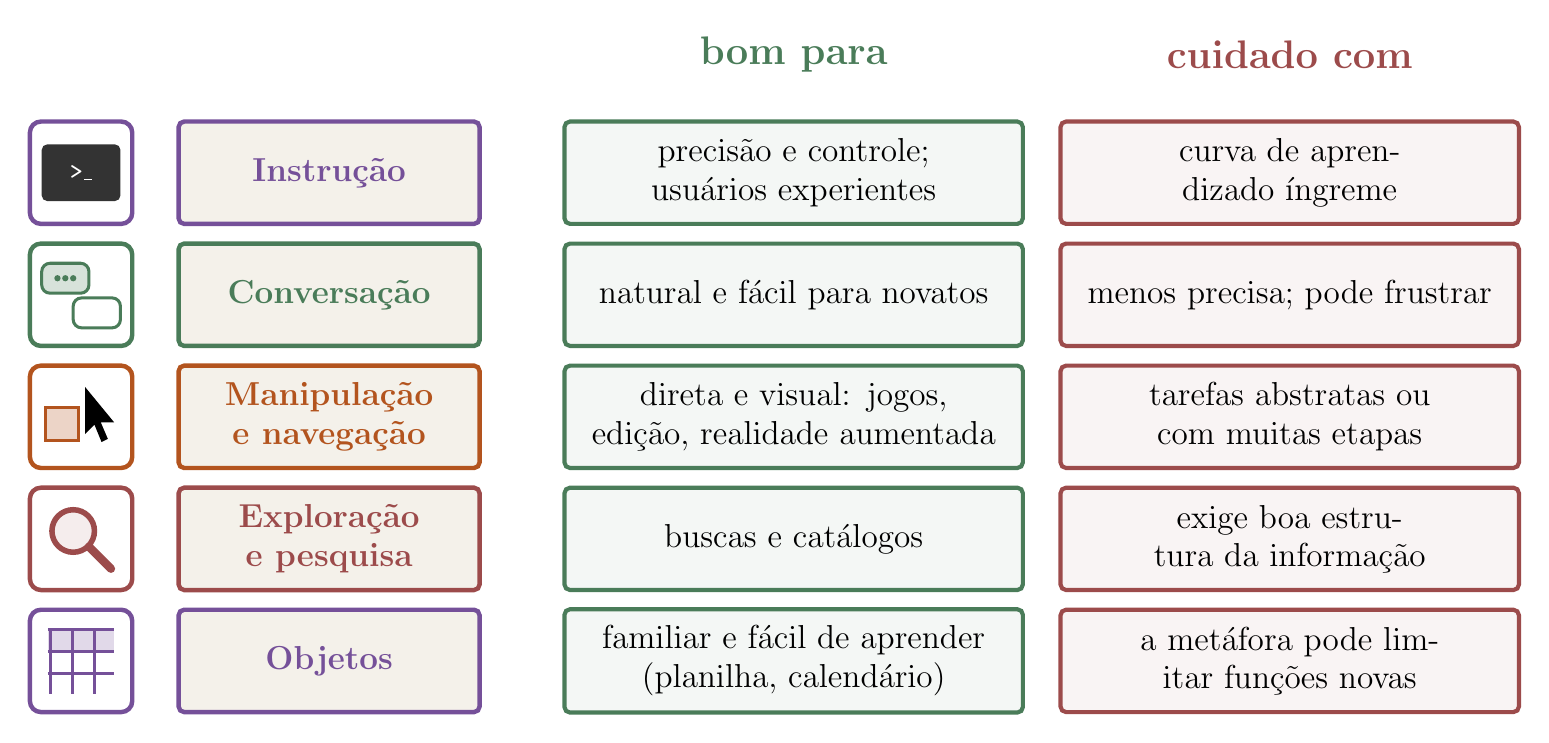
\begin{tikzpicture}[x=1cm,y=1cm]
\node[font=\Large\bfseries, dgreen] at (10.0,8.7) {bom para};
\node[font=\Large\bfseries, dred] at (16.3,8.7) {cuidado com};
\draw[dblue, fill=white, line width=1.6pt, rounded corners=4pt] (0.29999999999999993,6.55) rectangle ++(1.3,1.3);
\fill[black!80, rounded corners=2pt] (0.44999999999999996,6.84) rectangle (1.45,7.5600000000000005);
\node[white, font=\small\ttfamily] at (0.95,7.2) {>\_};
\node[dbox, draw=dblue, line width=1.6pt, text width=3.4cm, minimum height=1.3cm, font=\large\bfseries] at (4.1,7.2) {\textcolor{dblue}{Instrução}};
\node[dbox, draw=dgreen, fill=dgreen!6, line width=1.5pt, text width=5.4cm, minimum height=1.3cm, font=\large] at (10.0,7.2) {precisão e controle; usuários experientes};
\node[dbox, draw=dred, fill=dred!6, line width=1.5pt, text width=5.4cm, minimum height=1.3cm, font=\large] at (16.3,7.2) {curva de aprendizado íngreme};
\draw[dgreen, fill=white, line width=1.6pt, rounded corners=4pt] (0.29999999999999993,5.0) rectangle ++(1.3,1.3);
\draw[dgreen, fill=dgreen!22, line width=1.1pt, rounded corners=3pt] (0.44999999999999996,5.67) rectangle (1.05,6.050000000000001);
\draw[dgreen, fill=white, line width=1.1pt, rounded corners=3pt] (0.85,5.23) rectangle (1.45,5.61);
\fill[dgreen] (0.6499999999999999,5.86) circle (0.04) (0.75,5.86) circle (0.04) (0.85,5.86) circle (0.04);
\node[dbox, draw=dgreen, line width=1.6pt, text width=3.4cm, minimum height=1.3cm, font=\large\bfseries] at (4.1,5.65) {\textcolor{dgreen}{Conversação}};
\node[dbox, draw=dgreen, fill=dgreen!6, line width=1.5pt, text width=5.4cm, minimum height=1.3cm, font=\large] at (10.0,5.65) {natural e fácil para novatos};
\node[dbox, draw=dred, fill=dred!6, line width=1.5pt, text width=5.4cm, minimum height=1.3cm, font=\large] at (16.3,5.65) {menos precisa; pode frustrar};
\draw[dorange, fill=white, line width=1.6pt, rounded corners=4pt] (0.29999999999999993,3.4499999999999997) rectangle ++(1.3,1.3);
\draw[dorange, fill=dorange!25, line width=1.2pt] (0.49999999999999994,3.8) rectangle (0.9199999999999999,4.22);
\fill[black] (1.0,4.4799999999999995) -- (1.0,3.8799999999999994) -- (1.1199999999999999,3.9999999999999996) -- (1.21,3.78) -- (1.29,3.8199999999999994) -- (1.2,4.029999999999999) -- (1.3699999999999999,4.029999999999999) -- cycle;
\node[dbox, draw=dorange, line width=1.6pt, text width=3.4cm, minimum height=1.3cm, font=\large\bfseries] at (4.1,4.1) {\textcolor{dorange}{Manipulação e navegação}};
\node[dbox, draw=dgreen, fill=dgreen!6, line width=1.5pt, text width=5.4cm, minimum height=1.3cm, font=\large] at (10.0,4.1) {direta e visual: jogos, edição, realidade aumentada};
\node[dbox, draw=dred, fill=dred!6, line width=1.5pt, text width=5.4cm, minimum height=1.3cm, font=\large] at (16.3,4.1) {tarefas abstratas ou com muitas etapas};
\draw[dred, fill=white, line width=1.6pt, rounded corners=4pt] (0.29999999999999993,1.9) rectangle ++(1.3,1.3);
\draw[dred, fill=dred!10, line width=2pt] (0.85,2.65) circle (0.27);
\draw[dred, line width=3pt, line cap=round] (1.05,2.4499999999999997) -- (1.33,2.17);
\node[dbox, draw=dred, line width=1.6pt, text width=3.4cm, minimum height=1.3cm, font=\large\bfseries] at (4.1,2.55) {\textcolor{dred}{Exploração e pesquisa}};
\node[dbox, draw=dgreen, fill=dgreen!6, line width=1.5pt, text width=5.4cm, minimum height=1.3cm, font=\large] at (10.0,2.55) {buscas e catálogos};
\node[dbox, draw=dred, fill=dred!6, line width=1.5pt, text width=5.4cm, minimum height=1.3cm, font=\large] at (16.3,2.55) {exige boa estrutura da informação};
\draw[dblue, fill=white, line width=1.6pt, rounded corners=4pt] (0.29999999999999993,0.35) rectangle ++(1.3,1.3);
\fill[dblue!22] (0.53,1.1400000000000001) rectangle ++(0.84,0.28);
\draw[dblue, step=0.28, line width=1pt] (0.53,0.5800000000000001) grid ++(0.84,0.84);
\node[dbox, draw=dblue, line width=1.6pt, text width=3.4cm, minimum height=1.3cm, font=\large\bfseries] at (4.1,1.0) {\textcolor{dblue}{Objetos}};
\node[dbox, draw=dgreen, fill=dgreen!6, line width=1.5pt, text width=5.4cm, minimum height=1.3cm, font=\large] at (10.0,1.0) {familiar e fácil de aprender (planilha, calendário)};
\node[dbox, draw=dred, fill=dred!6, line width=1.5pt, text width=5.4cm, minimum height=1.3cm, font=\large] at (16.3,1.0) {a metáfora pode limitar funções novas};
\end{tikzpicture}
\end{document}
